% \documentclass[12p]{article}
\documentclass{article}
% bibliographystyle{seg asdf}
% \tiny\bibligoraphy{seq_eg} .bib file
% \usepackage[margin=1in, headheight=110pt]{geometry}
\usepackage[letterpaper, margin=1in]{geometry}
\usepackage{amssymb, amsmath, amsfonts, amsthm}
\usepackage{mathpazo}
\usepackage{setspace}
% \usepackage{probsoln}
\usepackage{fancyhdr}
\usepackage{hyperref}
\usepackage{float}
\usepackage{tikz}
\usepackage{enumitem}
\usepackage{listings}
% \usepackage{lipsum}
\usepackage{parskip} % Use for extra line spacing

\setlength{\parindent}{0 in}

% TODO change these when we figure them out
\newcommand{\name}{Flatlined}
% Flatlined
% Hoverwars
\newcommand{\team}{Team A --- Light Theme is for Heretics}
\newcommand{\botcount}{4}

% TODO change the placement of these?
\pagestyle{fancy}
\lhead{High-level Design}
\rhead{CPSC 585 --- Winter 2019}

\lfoot{\name{}}
\rfoot{\team{}}

\newenvironment{hangingpar}[1]
  {\begin{list}
          {}
          {\setlength{\itemindent}{-#1}%%'
           \setlength{\leftmargin}{#1}%%'
           \setlength{\itemsep}{0pt}%%'
           \setlength{\parsep}{\parskip}%%'
           \setlength{\topsep}{\parskip}%%'
           }
    \setlength{\parindent}{-#1}%%
    \item[]
  }
  {\end{list}}


\newcommand{\sep}{\;}
\newtheorem{theorem}{Theorem}
\theoremstyle{definition}
\newtheorem{definition}[theorem]{Definition}

\newcommand\floor[1]{\lfloor#1\rfloor}
\newcommand\ceil[1]{\lceil#1\rceil}
\begin{document}
\begin{titlepage}
  \begin{center}
    \vspace*{1cm}
    \Large{\textbf{University of Calgary}}\\
    \Large{\textbf{CPSC 585 --- Winter 2019 --- Games Programming}}\\
    \vfill
    \line(1,0){400}\\[1mm]
    \huge{\textbf{\name{}}}\\
    \large{\textbf{High-Concept Design Document}}\\
    \line(1,0){400}\\
    \vfill
    \Large{\textbf{\team{}}}\\
    \Large{Austin Easton, Evan Quan, James Cote, Jianan Ding}\\
    \large{January 21, 2019}
    % \today \\
  \end{center}
\end{titlepage}
% \thispagestyle{fancy}
\setcounter{page}{0}
\tableofcontents
\pagenumbering{gobble}
\break{}
\pagenumbering{arabic}
% \onehalfspacing

\section{Overview}

\name{} is a combat-based driving game aimed to test your skill to fight
against your enemies. Whether playing alone against AI or with friends, each
player find themselves driving a hovercraft in an arena pitted against each
other. Utilizing abilities, picking up power-ups, and the navigating the map,
everyone must destroy each other in a chaotic battle of strategy and wits
before the round is over.

\section{Gameplay}

\subsection{Terminology}

\textbf{Arena/Map:} The closed area where the game takes place.

\textbf{Ability:} The capabilities that a hovercraft can actively use.

\textbf{Bot:} An AI-controlled hovercraft. These hovercrafts are distinct from
player hovercrafts.

\textbf{Player:} The individuals playing the game. May also interchangeably
refer to the hovercrafts controlled by the players for the sake of brevity,
especially in relation to the AI-controlled hovercrafts.

\textbf{Power-up:} An item located on the map that can be picked up by a player
by coming into contact with it. Upon pick-up, the player receives a temporary
effect, usually beneficial.

\subsection{Player Count}

The game supports single and local multiplayer, allowing for 1 to 4 players.
Local multiplayer would be split-screen multiplayer and would require multiple
input devices (XBOX controllers).

\subsection{Player Goal}

The central goal of the game is to gain the highest score possible before the
round is over. Players have the following means to gain score:
\begin{itemize}
  \item Damaging other player hovercrafts, which can only be done in
    multiplayer. This can be through the use of abilities accessible to every
    player. Depending on the means by which enemies are damaged, various
    amount of points can be awarded, encouraging the player to make interesting
    plays.
  \item Destroying other player hovercrafts, which can only be done in
    multiplayer. If damage is done to a hovercraft's final hit point and it is
    destroyed, extra points are awarded.
  \item Destroying bots, which can be done in both single and multiplayer.
    These hovercrafts do not have all the abilities of player hovercrafts and
    so reward less points.
  \item Picking up power-ups. These help the player gain points by improving
    their abilities, but also innately give points when they are picked up.
\end{itemize}

\subsection{Rounds}

The game is composed of a single round that lasts for the duration of a timer.
Each player is placed in an arena to control a hovercraft with various
abilities. They must fight each other in a free-for-all battle with those
abilities, amidst a number of neutral bots for added chaos.

\subsection{Damage}

% TODO
Players start the game alive with a set amount of hit points, which will be
explicitly displayed to the player. They can be damaged by the abilities of
other hovercrafts, lowering their current hit points. When all hit points is
removed, the player's hovercraft is destroyed.

When a player's hovercraft is destroyed, they lose some points and are
momentarily out of the game before respawning randomly at one of the number of
respawn points on the map. If another player destroyed said hovercraft, that
player is awarded points for the kill.

Similar to \textbf{Mario Kart}'s battle mode, all sources of damage deal
a single point of damage. Hovercraft hit points are also a small, discrete value.
This emphases dodging and avoiding abilities, and eases player understanding of
how abilities work without needing to worry about different damage values.

% TODO promised features/low prio?
The central constraint of proposed features is development time available to
implement them. As a result, all features have an associated priority and risk,
of which higher priority features will be completed first, and higher risk
features will more likely be altered, replaced, or not implemented at all.

% TODO I can write a reasonably short one to set the scene if need be. Doesn't
% need to actually be included in the game.

\subsection{Arenas/Maps}

% TODO mention development time?
The game will feature a single map. Given the development time frame, a single
fun and polished map is preferable to multiple mediocre maps. It should be
``small'' to ``medium'' in size, to maintain a high player density to ensure
that players are always in the middle of the action, and do not get lost.

If time allows for additional maps, they may be added at a lower priority, but
the focus will still be on a singular main map. These additional maps should
provide a different purpose than the main map. For example, there could be
a small map focused for single player.
% TODO should be included? Tentative stuff? High-low priority stuff?

\textbf{Environmental features}

\begin{itemize}
  \item Ramps --- Ramps lead to higher and lower platforms, or can be jumped
    off of. This can provide better vision of certain parts of the map, give
    opportunities to jump between arenas.
  \item Lava pit --- Falling into the pit will destroy the player hovercraft.
    Avoid at all costs or try to bump enemies into it.
  \item Speed pads --- Driving over these, will give a momentary boost of
    speed. Great for getting power-ups quicker, and chasing or escaping other
    players.
\end{itemize}

\subsection{Bots}

In all modes, a number of neutral bots will be present on the map. Visually
distinct from players, bots will attempt to crash into the players to damage
them. They are weaker than players in that they have fewer hit points and fewer
abilities, but also award less points on kill. As a result, it is up to players
to decide much they want to focus on destroying bots versus other players in
their strategy.

\subsection{Abilities}

\textbf{Movement}

\begin{itemize}
  \item \textbf{Standard movement} --- A hovercraft does not rely on wheels to
    move and so can traverse in any lateral direction without needing to turn,
    meaning that strafing is possible.
  \item \textbf{Acceleration/braking} --- A hovercraft can accelerate an brake
    in any direction is it currently moving. It will often drift if a turn is
    made, even at relatively slow speeds, which can be both advantageous and
    disadvantageous.
  \item \textbf{Dashing} --- A hovercraft can dash in any direction,
    temporarily gaining invulnerability. From a mobility standpoint, dashing
    can be used to catch up to other hovercrafts, reach power-ups faster, or
    lose others when being chased. From a defensive standpoint, it can be used
    to dodge attacks.
\end{itemize}

\textbf{Attacks}

Every hovercraft has 3 attack abilities that are available from the start of
the game.

\begin{itemize}
  \item \textbf{Rocket} --- A rocket launches forward straight out from the
    direction the hovercraft is facing until it hits a surface. Upon impact, it
    explodes, damaging everything in a radius around it. Being the only ranged
    attack, it is great for attacking distant enemies if aimed well, or when
    chasing other vehicles. The splash damage can be utilized with parts of the
    arena environment to hit enemies near walls easier, or to hit multiple
    enemies that are grouped together.
  \item \textbf{Spikes} --- Spikes temporarily extend in all directions from
    the hovercraft, damaging other vehicles that come in contact with it. Can
    be used both aggressively and defensively when other vehicles are nearby.
    It can also be used in combination with dashing to crash into enemies.
  \item \textbf{Flame trail} --- A trail of fire is created that follows the
    players path. Any hovercraft that contacts it is damaged. Great to use when
    being chased.
\end{itemize}


\subsection{Power-Ups}

Power-ups spawn at certain explicit power-up locations, where players can pick
them up by contacting them. Upon contact, the player that picked it up will
receive a temporary passive bonus. At minimum, there will be a power-up for
each attack ability:
\begin{itemize}
  \item \textbf{Rocket} --- Rockets can be launched at a faster rate of fire.
  \item \textbf{Spikes} --- Create a temporary shield that blocks damage upon
    activation.
  \item \textbf{Flame trail} --- The trail continuously lasts for the duration
    of the power-up.
  \item \textbf{Repair} --- Gain an extra hit point
\end{itemize}

\subsection{Difficulty}

\textbf{Single Player}

In a single player experience, the difficulty can arise
from a competitive approach in achieving a high-score. Whether one is
attempting to outperform their previous high scores, or compete with others'
high scores, players can improve their skills and learn new strategies to
improve. This self-imposed motivation to improve and compete can create new
levels of difficulty at a meta game level.

\textbf{Multiplayer}

Similar to single player, difficulty arises from the skills of opposing
players. As other players improve, so does oneself need to do to so to compete.
New strategies can arise in using abilities, power-ups, and parts of the map to
maximize points, as well as strategies to counter other players' play styles.

\subsection{Menu}

\section{Game Design}

\subsection{Aesthetic Themes}

The game mainly follows a cyberpunk/TRON aesthetic.

\subsection{Inspiration}

\name{} at its core is inspired by \textbf{Mario Kart}'s battle mode. Abilities
and mechanics in the game are also inspired by \textbf{Tron} (1982),
\textbf{Rocket League} (2015), \textbf{ThinkTanks} (2003), and \textbf{Pac-Man}
(1980).

\subsection{Designer Insight/Goals}

Here are some goals we have in mind for the project, as well as some insight
behind our design decisions.

\subsubsection{Vibe}

Playing \name{} should feel exciting and bring a sense of hype and energy,
similar to combat games like \textbf{Super Smash Bros} or \textbf{Street
Fighter}. This can be brought about through fast-paced gameplay, coupled with
action-packed sound effects and music.

\subsubsection{Role of AI}

The introduction of AI-controlled hovercrafts (bots) adds an interesting
element to the game, but also a few problems.

First, given our past experience and the time-frame creating AI, we don't
believe the bots will be equally competent to a skilled human player. If bots
are given a hovercraft with equal capability to that of a player, it is
unlikely they will be able to utilize their abilities and movement sufficiently
to compete with players, or have sufficient game sense to outplay and counter
different play styles. This poses a problem for single-player, as competing
against a group of underperforming bots not particularly fun or challenging.

It is possible to give bots a point bonus to compensate for their simple
behaviour, which partly addresses the challenge issue by giving the bots
a higher chance to reach the highest score. However, this does not necessarily
address the fun issue, as the player will still experience fighting against
simple bots.

Instead, bots can be given an alternative role rather than replacing a player.
By explicitly giving them less capabilities than the player, and having them
exist in-game independent from the player count, they can add an extra depth to
the gameplay without heavily relying on the depth of their capabilities. The
benefit is that if the bots end up more capable than we initially planned, this
design decision still works and will simply make the gameplay more engaging.

% TODO add later
% The crux of the fun should be from the multiplayer experience and not depend on
% the capabilities of the AI.\@

\subsubsection{Driving System}

Since players are driving hovercrafts, the driving experience should model
that of a hovercraft. As a result, the driving model should feel somewhat
floaty, allowing for easier drifting. Without the constraint of wheels, the
players should be able to move in any lateral direction without needing to
turn, allowing for strafing.

However, if the hovercrafts are too floaty, they may be frustrating to control.
Driving needs to feel responsive, especially if sudden turns or braking are
done.

Our goal is for there to be a balance in the driving system for it to feel
somewhat floaty to imitate a hovercraft, and yet grounded enough to feel fun
and responsive.

\subsubsection{Learning Curve}

\textbf{Easy to Learn}

A core goal for game is for it to be easy to pick up and start playing.
Part of this involves controls that are intuitive to new players. While there
are a fair number of abilities, they are the same for everyone, meaning players
do not need to know the ins-and-outs of different vehicle abilities that they
themselves do not have access to.

Power-ups should feel intuitive to understand and use. They should not
introduce new mechanics or keybindings. It is frustrating for for new players
to ``waste'' power-ups in order to understand what they do, especially if they
are single-use. Instead, power-ups should augment already existing abilities
and clearly display in the UI which ability is improved.

\textbf{Hard to Master}

Players should be given opportunities to improve and apply their skill. Each
ability is distinct and requires its own skills to use.
% TODO

\subsubsection{Blue Shell Effect} % TODO balance?


\subsubsection{Performance}

\begin{itemize}
  \item \name{} should run at 60 fps for single player and 30 fps for
    multiplayer.
\end{itemize}


\subsection{Market Competition}

% TODO redo game competition
There are competitive elements to both the single-player and multiplayer
experience. In single-player, players can compete to achieve the highest score
possible, akin to competing to reach the top positions in the leader boards
in arcade games or certain online games. In other words, this can be be viewed
as a competitive asynchronous multiplayer experience.

In multiplayer, players can learn strategies to to counter 

\subsection{Game Genre} % Is this needed?

\name{} is a third-person combat-based driving game. It is designed to be
a fun party game that is easy for new players to pick up and play, while giving
the opportunity to those who want to master it the means to do so given.

It is developed for the PC, supporting Windows as a high priority and Mac and
Linux with lower priorities, using mouse and keyboard controllers. It will also
support XBOX 360 controller support, allowing for multiplayer modes.

\subsection{Branding}

\name{} is a new IP on its own.

\subsection{Target Market}

While violence is a core component of the gameplay, nothing is particularly
graphic due to the use of vehicles and the lack of blood and gore. We do not
intend there to be any mature themes in the game. We therefore believe that
\name{} is appropriately targeted for all ages 10 and above years of age.

\subsection{Gameplay Direction} % TODO needed?


\section{Concept Art}

\begin{figure}[htpb]
  \centering
  \includegraphics[width=0.8\linewidth]{Brainstorming_001.png}
  \caption{Rough sketches of the map, UI, and hovercraft}
  \label{fig:Brainstorming_001}
\end{figure}

\begin{figure}[htpb]
  \centering
  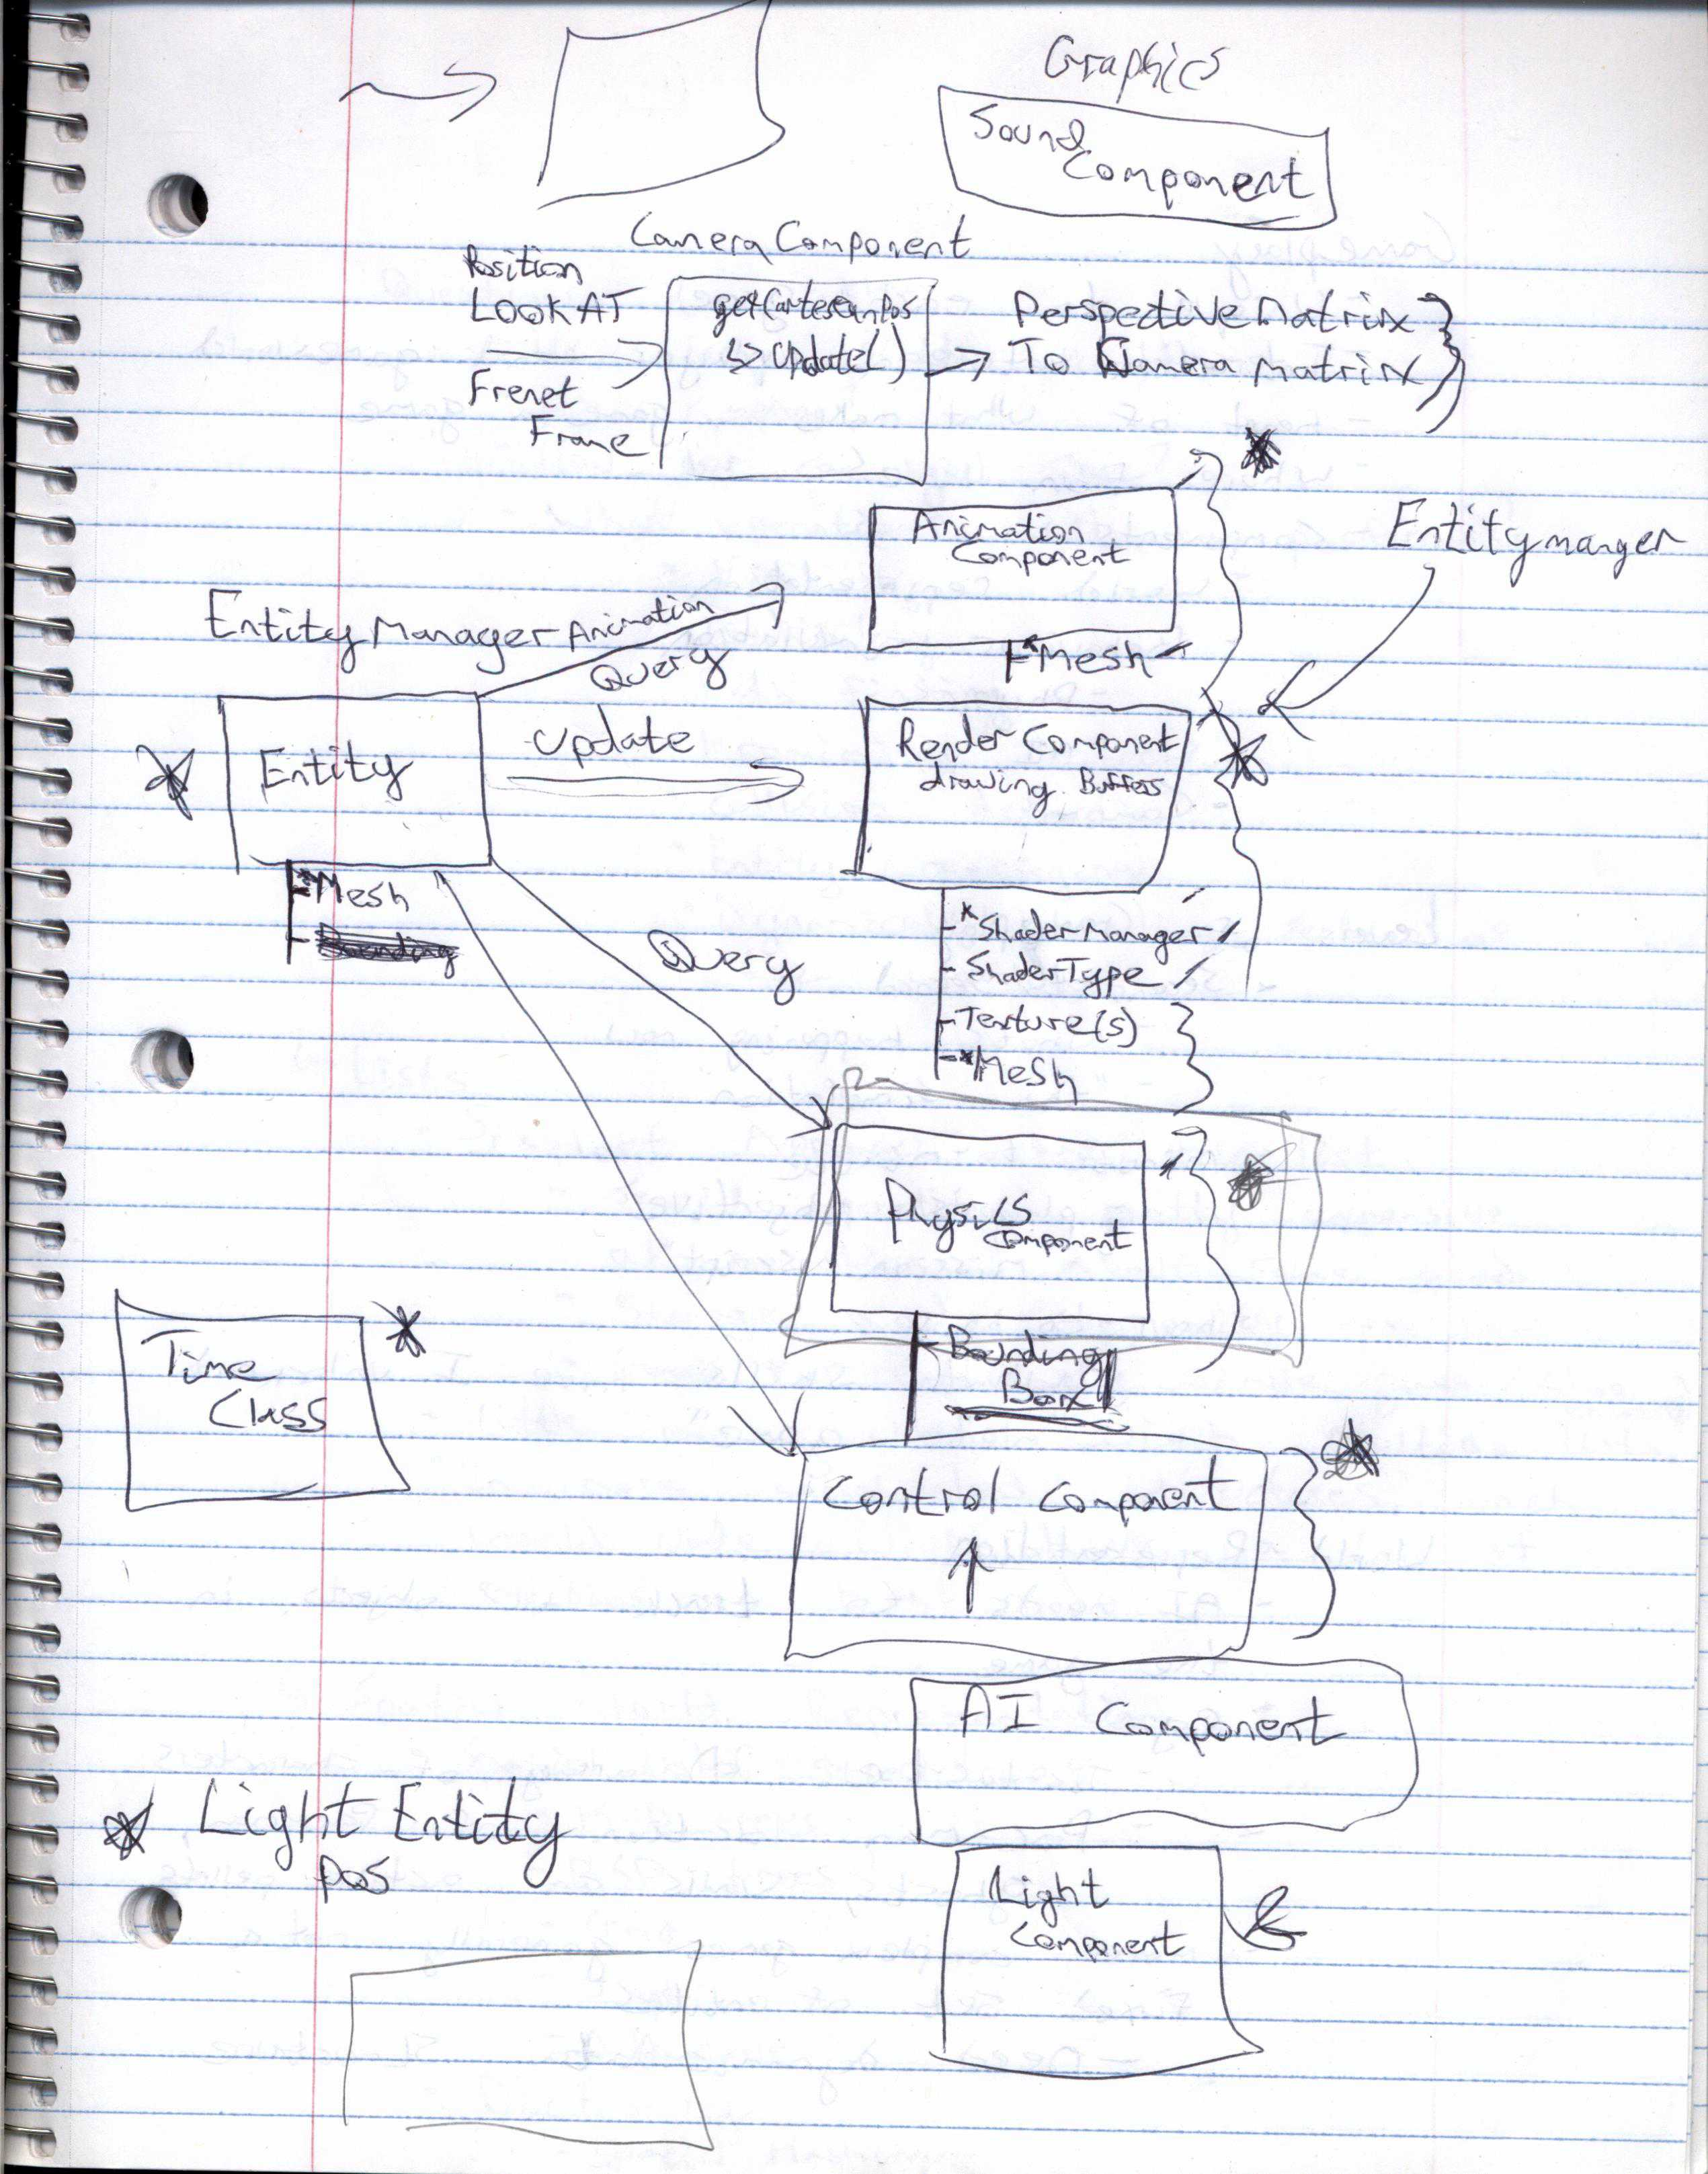
\includegraphics[width=0.8\linewidth]{Brainstorming_002.jpg}
  \caption{Early design of the game aplicaiton framework}
  \label{fig:Brainstorming_002}
\end{figure}

\begin{figure}[htpb]
  \centering
  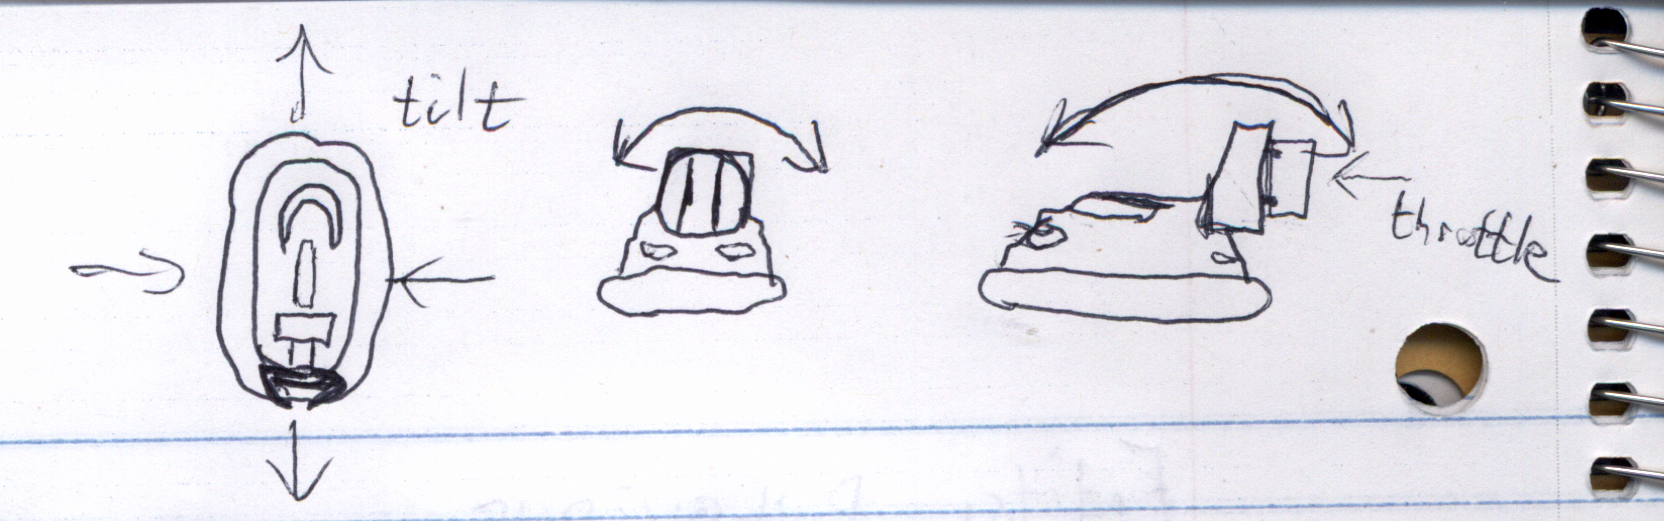
\includegraphics[width=0.8\linewidth]{Brainstorming_003.png}
  \caption{Sketch of hovercraft design}
  \label{fig:Brainstorming_003}
\end{figure}

\end{document}
